%\documentclass[german,10pt]{book}      
\usepackage{makeidx}
\usepackage{babel}            % Sprachunterstuetzung
\usepackage{amsmath}          % AMS "Grundpaket"
\usepackage{amssymb,amsfonts,amsthm,amscd} 
\usepackage{mathrsfs}
\usepackage{rotating}
\usepackage{sidecap}
\usepackage{graphicx}
\usepackage{color}
\usepackage{fancybox}
\usepackage{tikz}
\usetikzlibrary{arrows,snakes,backgrounds}
\usepackage{hyperref}
\hypersetup{colorlinks=true,
                    linkcolor=blue,
                    filecolor=magenta,
                    urlcolor=cyan,
                    pdftitle={Overleaf Example},
                    pdfpagemode=FullScreen,}
%\newcommand{\hyperref}[1]{\ref{#1}}
%
\definecolor{Gray}{gray}{0.80}
\DeclareMathSymbol{,}{\mathord}{letters}{"3B}
%
\newcounter{num}
\renewcommand{\thenum}{\arabic{num}}
\newenvironment{anmerkungen}
   {\begin{list}{(\thenum)}{%
   \usecounter{num}%
   \leftmargin0pt
   \itemindent5pt
   \topsep0pt
   \labelwidth0pt}%
   }{\end{list}}
%
\renewcommand{\arraystretch}{1.15}                % in Formeln und Tabellen   
\renewcommand{\baselinestretch}{1.15}                 % 1.15 facher
                                                      % Zeilenabst.
\newcommand{\Anmerkung}[1]{{\begin{footnotesize}#1 \end{footnotesize}}\\[0.2cm]}
\newcommand{\comment}[1]{}
\setlength{\parindent}{0em}           % Nicht einruecken am Anfang der Zeile 

\setlength{\textwidth}{15.4cm}
\setlength{\textheight}{23.0cm}
\setlength{\oddsidemargin}{1.0mm} 
\setlength{\evensidemargin}{-6.5mm}
\setlength{\topmargin}{-10mm} 
\setlength{\headheight}{0mm}
\newcommand{\identity}{{\bf 1}}
%
\newcommand{\vs}{\vspace{0.3cm}}
\newcommand{\noi}{\noindent}
\newcommand{\leer}{}

\newcommand{\engl}[1]{[\textit{#1}]}
\parindent 1.2cm
\sloppy

         \begin{document}  \setcounter{chapter}{2}

\chapter{Die Zeitgleichung}
% Kap 3
\label{chap_Zeitgleichung}

Die sogenannten \textit{wahren Sonnentage},\index{wahrer Sonnentag}\index{Tag!wahrer Sonnentag} 
hier ist die Zeitdauer von Sonnenh\"ochststand bis zum n\"achsten Sonnenh\"ochststand
gemeint, sind nicht immer gleich lang. Daf\"ur sind in erster Linie zwei Einfl\"usse verantwortlich:
die elliptische Form der Erdbahn und die Neigung der Erdachse gegen die 
Ekliptik, also die Ebene, in der die Erdbahn um die Sonne verl\"auft. Dies f\"uhrt zu einer 
Differenz zwischen der wahren Sonnenzeit\index{Sonnenzeit!wahre}\index{Sonnenzeit!mittlere} 
(bei der die Sonne um 12 Uhr ihren H\"ochststand
in Richtung S\"uden erreicht) und der sogenannten mittleren Sonnenzeit, wie sie auf einer 
gleichm\"a\ss ig gehenden Uhr angezeigt wird.\footnote{Hinzu kommt noch, dass die Ortszeit heute
nicht mehr die wahre Ortszeit ist, sondern einer Zeitzone zugeteilt wurde. Je nach L\"angengrad, an
dem sich ein Ort befindet, muss zur lokalen Zeit entsprechend der Zeitzone noch ein Korrekturterm
hinzugef\"ugt werden werden. Diese Korrektur wird in Abschnitt \ref{sec_wahrerSonnentag} kurz 
erw\"ahnt und ansonsten nicht ber\"ucksichtigt.}
Diese Differenz, die sogenannte Zeitgleichung,\index{Zeitgleichung} 
war schon im Altertum bekannt. Die Zeitgleichung ${\rm ZG}(t)$ gibt an, wie viele Minuten man zur gemessenen 
wahren Ortszeit addieren muss, um die gemittelte Ortszeit zu erhalten:
\begin{equation}
       {\rm ZG}(t) = \mbox{Mittlere Ortszeit}(t) - \mbox{Wahre Ortszeit}(t) \, .
\end{equation}
Sie konnte auf der Basis der Kepler'schen Gesetze Anfang des 16.\ Jahrhunderts auch theoretisch
begr\"undet werden. 

In Tabelle \ref{tab_Zeit} sind die wichtigsten Gr\"o\ss en zusammengefasst, die in diesem
Kapitel ben\"otigt werden.\index{Halbachse!Erde-Sonne}\index{Perihel}\index{Erdachse!Neigung zur Ekliptik}%
\index{Ekliptik}\index{Exzentrizit\"at!Erdbahn}\index{Sonne!Abstand}\index{Jahr!tropisches}

\begin{table}[htb]
\begin{tabular}{r|l}
gro\ss e Halbachse Erde-Sonne &  $a = 149\,598\,023$\,km   \\
Datum des Perihels &  derzeit am $(3\pm 2)$. Januar \\
Neigung der Erdachse zur Ekliptik&   $\varepsilon = 23,44^\circ $  \\
numerische Exzentrizit\"at der Erdbahn & $\epsilon = 0,0167$ \\
Abstand Erde-Sonne im Perihel & $r_{\rm min} = 147,10 \cdot 10^6\,{\rm km}$ \\  
Abstand Erde-Sonne im Aphel & $r_{\rm max} = 152,10 \cdot 10^6\,{\rm km}$ \\  
Dauer eines tropischen Jahres & $365,24219$\,Tage \\ 
\end{tabular}
\caption{\label{tab_Zeit}%
Die wichtigsten physikalischen Gr\"o\ss en im Zusammenhang mit der
Zeitgleichung. Je nach Zusammenhang und erforderlicher Genauigkeit werden die Werte 
unterschiedlich gerundet.}
\end{table}


\section{Zeitsysteme}

Wie schon erw\"ahnt, entspricht der Sonnenstand, die sogenannte wahre
Sonnenzeit, im Allgemeinen nicht dem, was man als Ortszeit bezeichnet. 
Zum einen hat es sich als sinnvoll erwiesen, sogenannte Zeitzonen zu definieren,
innerhalb deren die Zeitsysteme gleich sind, zum anderen ist der scheinbare Gang der Sonne
am Himmel nicht vollkommen gleichf\"ormig.\index{Zeitzone} 

\subsection{Zeitzonen}

Die wahre Sonnenzeit an einem bestimmten Ort auf der Erde ist definiert durch
den Sonnenh\"ochststand, der den Zeitpunkt 12 Uhr festlegt. Auf der
n\"ordlichen Halbkugel (n\"ordlich des $23,5$.\ Breitengrads) befindet sich die
Sonne in diesem Augenblick genau im S\"uden, auf der s\"udlichen Halbkugel (s\"udlich
des $-23,5$.\ Breitengrads) ist sie im Norden.\footnote{Zwischen diesen Breitengraden
kann die Sonne zu diesem Zeitpunkt je nach Jahreszeit im Norden oder S\"uden 
stehen. In jedem Fall entspricht ihre Lage einem Extrempunkt bez\"uglich des
Winkels \"uber dem Horizont.}  
Etwas anders ausgedr\"uckt handelt es sich bei 12 Uhr mittags (wahre Sonnenzeit) um
den Augenblick, an dem die Verbindungslinie Erdmittelpunkt-Sonnenmittelpunkt den
L\"angengrad des jeweiligen Orts schneidet. Ein wahrer Sonnentag ist dann der
Zeitraum von einem Sonnenh\"ochststand zum n\"achsten Sonnenh\"ochststand.

Die wahre Uhrzeit (bez\"uglich der Sonne) h\"angt vom L\"angengrad eines Orts ab.
Aus diesem Grund ist eine solche Zeitrechnung sehr kompliziert, da sie lokal von Ort zu Ort
verschieden sein kann. Bis zum Ende des 19.\ Jahrhunderts war das tats\"achlich der Fall:
Jede gr\"o\ss ere Stadt hatte ihre eigene Ortszeit. Insbesondere als Folge des
zunehmenden Eisenbahnverkehrs wurde ein solches System jedoch zu
umst\"andlich, und so wurde per Erlass im Jahre 1893 in Deutschland als gesetzliche
Zeit die Zeit am 15.\ L\"angengrad eingef\"uhrt. Diese Zeit bezeichnet man allgemein
auch als \glqq Mitteleurop\"aische Zeit (MEZ)\grqq, da\index{MEZ, mitteleurop\"aische Zeit} 
sie in den meisten europ\"aischen L\"andern gilt.\index{Zeitzone!MEZ} 

\begin{figure}[htb]
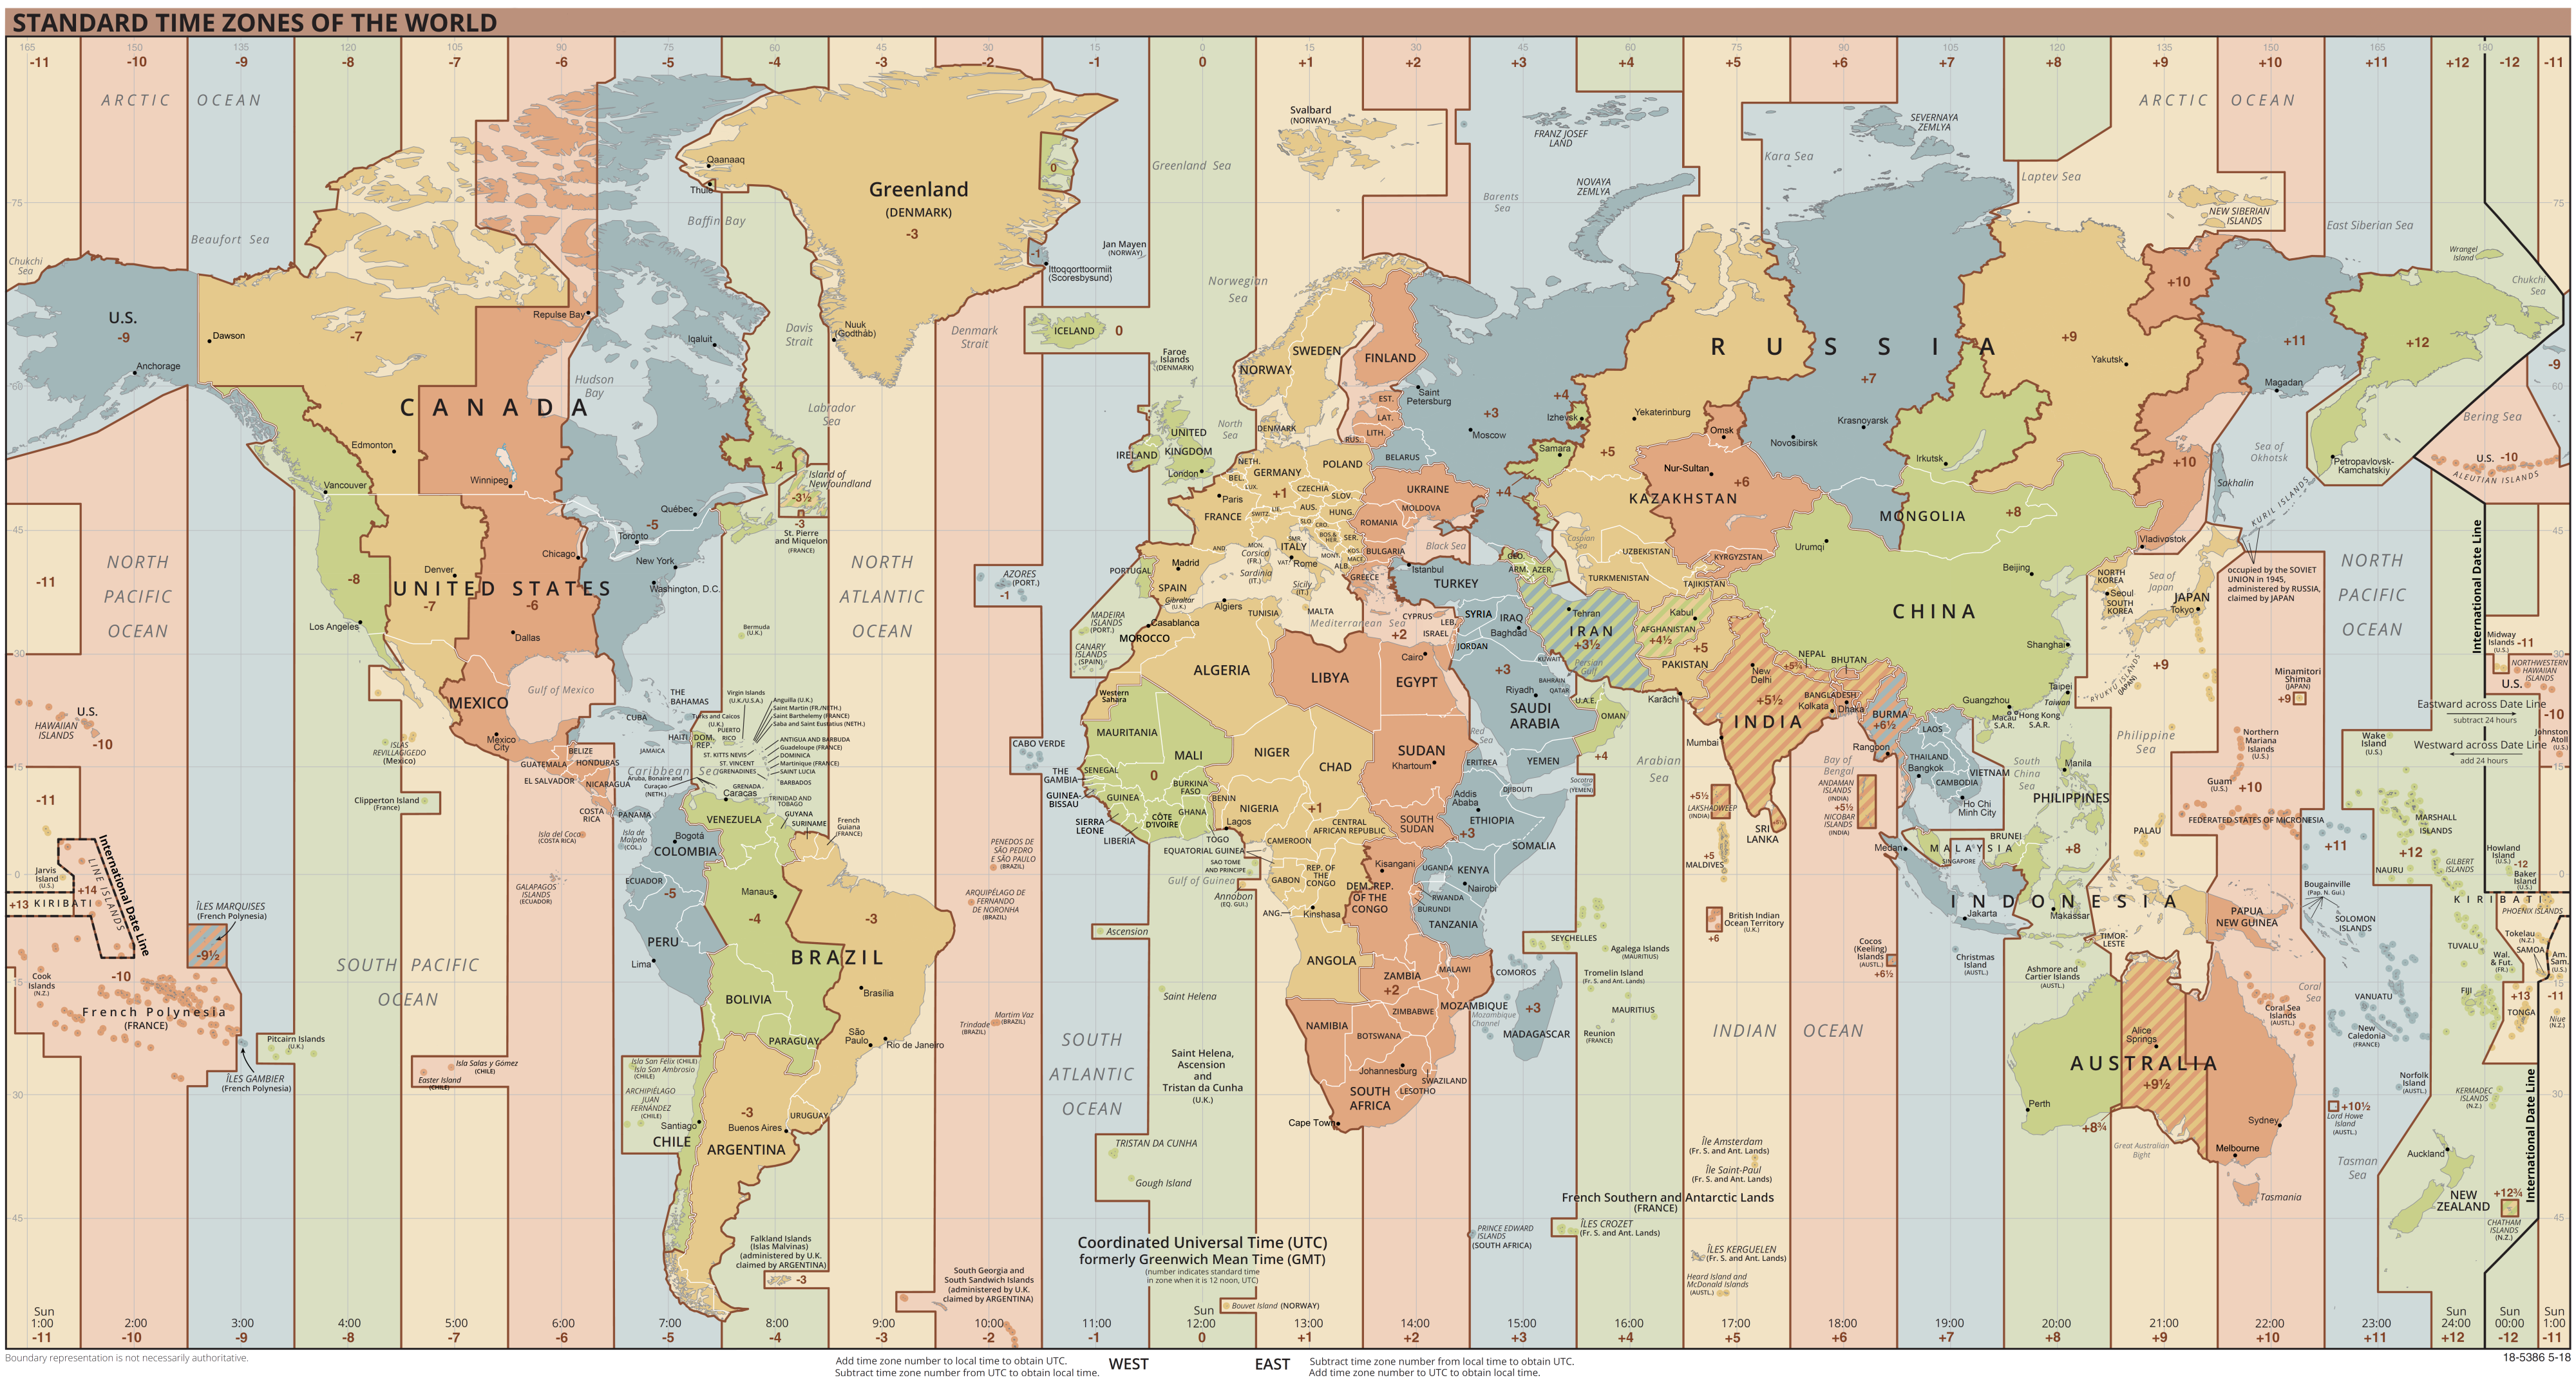
\includegraphics[scale=0.18]{./Bilder/World_Time_Zones_Map.png}
\caption{\label{fig_Zeitzonen}%
Die Zeitzonen der verschiedenen L\"ander. (aus \cite{Wikipedia_Zeitzone})}
\end{figure}

Die Erdkugel ist in 24 Zeitzonen eingeteilt (Abb.\ \ref{fig_Zeitzonen}), jede Zeitzone umfasst 
somit $360/24=15$ L\"angengrade. Befindet sich ein Ort nicht auf dem L\"angengrad seiner Zeitzone, muss 
man pro L\"angengraddifferenz 4 Minuten addieren bzw.\ subtrahieren, je nachdem ob sich der
Ort westlich oder \"ostlich von dem L\"angengrad seiner Zeitzone befindet. Die Mitteleurop\"aische
Zeit, die in Deutschland und den meisten westeurop\"aischen Kontinentalgebieten (au\ss er Portugal)
g\"ultig ist, hat ihren L\"angengrad bei $15^\circ$ Ost. Das ist nahe des
\"ostlichsten Punkts der deutschen Grenze. Selbst Frankfurt an der Oder liegt noch etwas weiter
westlich. Freiburg\index{Freiburg!Zeitzone} 
liegt beim L\"angengrad $7,85^\circ$, also $7,15^\circ$ westlich vom 15.\
L\"angengrad. Dementsprechen muss man zur MEZ rund 28,6 Minuten addieren, um die
wahre Ortszeit zu erhalten (in der Sommerzeit nochmals eine Stunde mehr). Der Sonnenh\"ochstand
im Sommer in Freiburg ist gegen 13:30.   

\subsection{Wahrer und mittlerer Sonnentag}
\label{sec_wahrerSonnentag}

Unabh\"angig von den bisher erw\"ahnten Korrekturen, die zur Bestimmung der lokalen
Ortszeit notwendig sind, kann der wahre Sonnentag, also die Zeitdauer zwischen zwei 
Sonnenh\"ochstst\"anden an einem Ort, im Laufe eines Jahres um bis zu fast einer halben Minute
schwanken, was sich zu manchen Zeiten kumulativ bis zu einer Viertelstunde aufaddieren kann. 
Die beiden Hauptursachen daf\"ur - die elliptische Bahn der Erde und die Neigung der Erdachse 
relativ zur Ekliptik - werden in den Abschnitten \ref{sec_Ellipse} und \ref{sec_Neigung} besprochen. 
Aus diesem Grund definiert man einen mittleren Sonnentag\index{Sonnentag!wahrer} 
als die Dauer eines Tages, sodass ein Jahr\index{Sonnentag!mittlerer}
genau $365,2422$ mittlere Sonnentage hat. Dies hat jedoch zur Folge, dass eine
Uhr, welche die Uhrzeit nach dem mittleren Sonnentag anzeigt, nicht mit einer Uhr \"ubereinstimmt,
welche die wahre Sonnenzeit anzeigt, also z.B.\ eine Sonnenuhr.\index{Sonnenuhr} 
Manche Sonnenuhren
ber\"ucksichtigen diese Effekte, indem die Stundenlinien die Form eines sogenannten
Analemmas haben (Abschnitt \ref{sec_Analemma}).

\section{Zur Mathematik einer elliptischen Bahnkurve}

Es gibt zwei bekannte Definitionen einer Ellipse:\index{Ellipse} 
(1) als die Menge aller Punkte, bei denen die\index{Brennpunkt}
Summe der Abst\"ande zu zwei gegebenen Punkten, den Brennpunkten der Ellipse, konstant ist, 
und (2) als Schnitt
eines Kegelmantels mit einer Ebene. Dass die L\"osungen des Zwei-K\"orper-Kepler-Problems
(also das Zwei-K\"orper-Problem mit einem Potenzial proportional zu $1/r$) Kegelschnitte
sind, ist ebenfalls bekannt. Die gebundenen L\"osungen bilden dabei Ellipsen, wobei 
der Kreis ein Spezialfall einer Ellipse ist. 

Die sogenannte \textit{lineare Exzentrizit\"at} $e$\index{Exzentrizit\"at!lineare} 
einer Ellipse ist gleich dem Abstand vom 
Mittelpunkt der Ellipse zu einem der Brennpunkte. Sie hat die Dimension einer L\"ange. 
Die \textit{numerische Exzentrizit\"at}\index{Exzentrizit\"at!numerische} 
$\epsilon$ ist gleich dem Verh\"altnis von $e$ zur gro\ss en
Halbachse $a$ und ist somit dimensionslos (vgl.\ Abb.\ \ref{fig_ellipse}, links):
\begin{equation}
\label{eq_fracea}
               \epsilon = \frac{e}{a} \, .
\end{equation}
Au\ss erdem gilt
\begin{equation}
\label{eq_zweia}
             2a = r_{\rm max} + r_{\rm min}  \hspace{1cm} {\rm und} \hspace{1cm}
             2e = r_{\rm max} - r_{\rm min}   \, ,
\end{equation}
wobei $r_{\rm max}$ der maximale Abstand zwischen einem Brennpunkt und der Ellipse ist (also der
Abstand zwischen einem Brennpunkt und dem gegen\"uberliegenden Punkt der Ellipse) und $r_{\rm min}$
der minimale Abstand. Bei der Erdumlaufbahn um die Sonne bezeichnet man den Punkt mit dem
maximalen Abstand zur Sonne als Aphel,\index{Aphel}\index{Perihel} 
den Punkt mit dem minimalen Abstand als Perihel.\footnote{Bei der Mondbahn 
um die Erde bezeichnet man den Punkt der Mondbahn mit dem gr\"o\ss ten 
Abstand zur Erde als Apog\"aum\index{Apog\"aum}\index{Perig\"aum} 
und den Punkt mit dem kleinsten Abstand als Perig\"aum.} 
 
Aus den Gleichungen \ref{eq_fracea} und \ref{eq_zweia} folgt
\begin{equation}
               \epsilon = \frac{r_{\rm max} - r_{\rm min}}{r_{\rm max} + r_{\rm min}}
               \hspace{1cm}  {\rm oder}  \hspace{1cm}   \frac{r_{\rm min}}{r_{\rm max}} = 
               \frac{1-\epsilon}{1+\epsilon}         \, .
\end{equation}

\begin{figure}[htb]
\setlength{\unitlength}{0.8pt}
\begin{picture}(250,150)(8,0)
\qbezier(8.5,75)(9,107)(50,130)
\qbezier(50,130)(80,145)(125,146)
\qbezier(8.5,75)(9,43)(50,20)
\qbezier(50,20)(80,5)(125,4)
\qbezier(241.5,75)(241,107)(200,130)
\qbezier(200,130)(170,145)(125,146)
\qbezier(241.5,75)(241,43)(200,20)
\qbezier(200,20)(170,5)(125,4)
\put(53,75){\makebox(0,0){$\bullet$}}
\put(125,146){\makebox(0,0){$\bullet$}}
\put(197,75){\makebox(0,0){$\bullet$}}
\put(125,75){\makebox(0,0){$\bullet$}}
\put(8.5,75){\line(1,0){116.5}}
\put(125,75){\line(1,0){116.5}}
\put(53,75){\line(1,1){70}}
\put(197,75){\line(-1,1){70}}
\put(160,120){\makebox(0,0){$a$}}
\put(160,80){\makebox(0,0){$e$}}
%
\qbezier(8.5,73)(8.5,70)(20,70)
\qbezier(20,70)(31.5,70)(31.5,67)
\qbezier(31.5,67)(31.5,70)(43,70)
\qbezier(43,70)(53,70)(53,73)
\qbezier(53,73)(53,55)(120,55)
\qbezier(120,55)(150,55)(150,50)
\qbezier(150,50)(150,55)(180,55)
\qbezier(180,55)(241.5,55)(241.5,73)
\qbezier(125,73)(125,70)(153,70)
\qbezier(153,70)(180,70)(180,65)
\qbezier(180,65)(180,70)(207,70)
\qbezier(207,70)(241.5,70)(241.5,73)
\put(31.5,62){\makebox(0,0){$r_{\rm min}$}}
\put(150,45){\makebox(0,0){$r_{\rm max}$}}
\put(180,60){\makebox(0,0){$a$}}
\end{picture}
\hfill
\begin{picture}(270,150)(0,0)
\qbezier(8.5,75)(9,107)(50,130)
\qbezier(50,130)(80,145)(125,146)
\qbezier(8.5,75)(9,43)(50,20)
\qbezier(50,20)(80,5)(125,4)
\qbezier(241.5,75)(241,107)(200,130)
\qbezier(200,130)(170,145)(125,146)
\qbezier(241.5,75)(241,43)(200,20)
\qbezier(200,20)(170,5)(125,4)
\put(53,75){\makebox(0,0){$\bullet$}}
%\put(125,146){\makebox(0,0){$\bullet$}}
%\put(197,75){\makebox(0,0){$\bullet$}}
%\put(125,75){\makebox(0,0){$\bullet$}}
\put(8.5,73){\vector(0,-1){0}}
\put(241.5,77){\vector(0,1){0}}
\put(53,75){\line(-1,0){45}}
\put(53,75){\line(-2,-1){40}}
\put(53,75){\line(1,0){190}}
\qbezier(53,75)(147,80)(240,85)
%\qbezier(53,75)(147,70)(240,65)
\put(-9,75){\makebox(0,0){$v_{\rm max}$}}
\put(258,75){\makebox(0,0){$v_{\rm min}$}}
%
\put(55,55){\makebox(0,0){${\scriptstyle \alpha_{\rm max}}$}}
\put(55,60){\vector(-1,1){13}}
\qbezier(35,75)(35,70)(37,68)
\put(70,95){\makebox(0,0){${\scriptstyle \alpha_{\rm min}}$}}
\put(75,89.5){\vector(1,-1){13}}
\qbezier(120,75)(120,76)(119.5,79)
\put(33,81){\makebox(0,0){$r_{\rm min}$}}
\put(170,69){\makebox(0,0){$r_{\rm max}$}}
\end{picture}
\caption{\label{fig_ellipse}%
(links) Die geometrischen Gr\"o\ss en in einer Ellipse: $a$ (gro\ss e Halbachse), $e$ (Exzentrizit\"at),
$r_{\rm min}$ und $r_{\rm max}$ (kleinster und gr\"o\ss ter Abstand der Ellipse zu einem Brennpunkt);
(rechts) die dynamischen Gr\"o\ss en in einer Ellipse: $v_{\rm min}$ und $v_{\rm max}$ (kleinste und
gr\"o\ss te Geschwindigkeit eines umlaufenden Objekts), $\alpha_{\rm max}$ und $\alpha_{\rm min}$ 
(in gleichen Zeiten \"uberstrichene Winkel im Perihel und Aphel).}
\end{figure}

Nach dem zweiten\index{Kepler'sches Gesetz!zweites} 
Kepler'schen Gesetz (\glqq In gleichen Zeiten werden gleiche Fl\"achen \"uberstrichen\grqq)
folgt, dass sich die Geschwindigkeiten im Perihel (dem sonnenn\"achsten Punkt), $v_{\rm max}$, 
zur Geschwindigkeit im Aphel (dem sonnenfernsten Punkt), $v_{\rm min}$, wie die Abst\"ande der Bahn
zur Sonne verhalten (siehe Abb.\ \ref{fig_ellipse}, rechts):
\begin{equation}
                 \frac{v_{\rm min}}{v_{\rm max}} =  \frac{r_{\rm min}}{r_{\rm max}}   \, .
\end{equation} 
Das zweite Kepler'sche Gesetz\index{Drehimpulserhaltung} 
ist \"aquivalent zur Drehimpulserhaltung.\hyperref[sec_Zeitgleichung_A]{(Herleitung)}

F\"ur die Winkel im Perihel $\alpha_{\rm max}$ und Aphel $\alpha_{\rm min}$, 
die in gleichen Zeiten \"uberstrichen werden, bedeutet dies:
\begin{equation}
\label{eq_maxzumin}
      \frac{\alpha_{\rm min}}{\alpha_{\rm max}} 
      = \left( \frac{v_{\rm min}}{r_{\rm max}} \right) \Big/ \left( \frac{v_{\rm max}}{r_{\rm min}} \right) 
                 = \left( \frac{r_{\rm min}}{r_{\rm max}} \right)^2 \, .
\end{equation} 

\section{Der Einfluss der elliptischen Bahnkurve}
\label{sec_Ellipse}

In diesem Abschnitt vernachl\"assigen wir die Neigung der Erdachse zur Ekliptik (diesen
Effekt ber\"ucksichtigen wir im n\"achsten Abschnitt) und nehmen an, die Rotationsachse
der Erde sei senkrecht zu ihrer Bahnebene. 

W\"urde sich die Erde auf einer Kreisbahn um die Sonne bewegen, w\"are der Winkel, den
sie auf ihrer Bahn um die Sonne t\"aglich \"uberstreicht, immer derselbe. Wir bezeichnen diesen Winkel
mit $\alpha_0$. Sein Wert berechnet sich aus der Tatsache, dass ein Jahr rund $365,2422$ Tage
dauert und in dieser Zeit ein Winkel von $360^\circ$ \"uberstrichen wird:
\begin{equation}
                \alpha_0 = \frac{360^\circ}{365,2422\,{\rm d}} = 0,98565^\circ/{\rm d} \, . 
\end{equation} 
Die Erde dreht sich in 24 Stunden einmal um ihre Achse von Sonnenh\"ohststand zu
Sonnenh\"ochstand. Dabei \"uberstreicht sie einen Winkel von 
$360^\circ + \alpha$. Der zus\"atzliche Winkel $\alpha$ r\"uhrt daher, dass sich die Erde im
Verlauf eines Tages auf ihrer Bahn weiter um die Sonne bewegt hat, und sich somit
die Sonne relativ zur Erde um den Winkel $\alpha$ weiterbewegt hat. Auf einer
Kreisbahn w\"are dieser Winkel $\alpha=\alpha_0$. Um sich um diesen Winkel $\alpha$
zu drehen, ben\"otigt sie ungef\"ahr 4 Minuten.\footnote{Da sich die Erde in 24 Stunden um
rund $360^\circ$ dreht, dreht sie sich in einer Stunde um $15^\circ$ und somit in 4 Minuten
um $1^\circ$.} 
Um diese Zeit ist der ideale Sonnentag\index{Tag!siderischer}
l\"anger als der siderische Tag (der sich auf eine Umdrehung relativ zum Fixsternhimmel bezieht).

Tats\"achlich bewegt die Erde sich aber auf einer elliptischen Bahn und ihre Winkelgeschwindigkeit
ist im Perihel gr\"o\ss er als im Aphel. Das bedeutet, dass an einem Tag in Periheln\"ahe (dieser Tag
liegt derzeit um den 3.\ Januar) ein gr\"o\ss erer Winkel von ihr relativ zur Sonne \"uberstrichen wird
als an einem Tag im Aphel (rund 3. Juli). F\"ur die Zeitabh\"angigkeit dieses Winkels k\"onnen wir
folgenden Ansatz machen
\begin{equation}
\label{eq_alphat}
                \alpha(t) = \alpha_0 \left( 1 + A \cos \left( \frac{2\pi}{T} t \right) \right)  \, , 
\end{equation} 
wobei $T$ die Periodendauer der Erdbahn um die Sonne ist - also ein Jahr -
und die Zeit $t$ am Perihel beginnen soll (also $\alpha(t=0)=\alpha_{\rm max}$). 
Nach Gl.\ \ref{eq_maxzumin} besteht folgende Beziehung zwischen der Amplitude $A$ und
der Exzentrizit\"at $\epsilon$: 
\begin{equation}
               \frac{\alpha_{\rm max}}{\alpha_{\rm min}} = \left( \frac{  1 + \epsilon}{1-\epsilon} \right)^2
              \approx 1+4\epsilon  \, . 
\end{equation} 
Andererseits gilt nach Gl.\ \ref{eq_alphat}:
\begin{equation}
               \frac{\alpha_{\rm max}}{\alpha_{\rm min}} =
            \frac{\alpha(0)}{\alpha(T/2)} = \frac{ \alpha_0 ( 1 + A )}{\alpha_0(1-A)} 
            \approx 1 + 2A  \, . 
\end{equation} 
Wir erhalten somit die Beziehung $A = 2 \epsilon$. 

F\"ur die Winkelgeschwindigkeit der Eigendrehung der Erde k\"onnen wir nach obiger
Argumentation schreiben:
\begin{equation}
             \omega = \frac{360^\circ + \alpha_0}{86400\,{\rm s}} \, .
\end{equation}
Andererseits ist die Zeitdauer $T(\alpha)$, die die Erde ben\"otigt, um sich um den Winkel
$\alpha$ zu drehen, gegeben durch
\begin{equation}
             T(\alpha)  = \frac{\alpha}{\omega}     \, , 
\end{equation} 
und damit dauert ein Tag (in Abh\"angigkeit von der Jahreszeit $t$):
\begin{eqnarray}
              T(t) &=& \frac{360^\circ + \alpha(t)}{\omega} 
              = \left( \frac{360^\circ + 
                   \alpha_0( 1 + 2 \epsilon \cos \frac{2\pi}{T}t)}{360^\circ + \alpha_0}\right)  T_0 \\
              &=& T_0 + 2 \alpha_0 \epsilon \frac{\cos  \frac{2\pi}{T}t}{360^\circ + \alpha_0} T_0  \, ,
\end{eqnarray} 
wobei $T_0=86\,400$\,s einem mittleren Sonnentag entspricht.
Die Zeitdifferenz zwischen einem mittleren Sonnentag und dem tats\"achlichen Sonnentag ist
somit
\begin{equation}
\label{eq_Zeitdifferenz}
              \Delta T(t) = T(t)-T_0 =  2 \alpha_0 \epsilon \frac{\cos  \frac{2\pi}{T}t}{360^\circ + \alpha_0}T_0   \, .
\end{equation} 
Setzen wir Werte ein, so erhalten wir f\"ur die Amplitude dieser Schwankung:
\begin{equation}
              \Delta T =  2 \alpha_0 \epsilon \frac{1}{360^\circ + \alpha_0} 86400\,{\rm s} \approx 
                7,88\,{\rm s}   \, .
\end{equation} 
Um diesen Wert kann ein einzelner Tag also l\"anger oder k\"urzer sein als ein mittlerer Sonnentag (sofern
man nur die elliptische Bahn der Erde ber\"ucksichtigt). Ein solcher Effekt f\"ur sich genommen w\"are vermutlich
im Altertum noch nicht aufgefallen, w\"are dieser Effekt nicht kumulativ, d.h., wenn viele aufeinanderfolgende
Tage um \"ahnliche Werte zu lang oder zu kurz sind, addieren sich die Effekte auf. Je nach Jahreszeit
geht die tats\"achliche
Zeit der gemittelten Zeit voraus bzw.\ nach. Relevant f\"ur die Zeitgleichung ist dieser kumulative
Effekt, d.h.\ die Differenz zwischen der wahren Zeit, die an einem Ort am Stand der Sonne abgelesen 
wird, und der gemittelten Zeit, die eine Uhr anzeigt. 

Bilden wir von Gl.\ \ref{eq_Zeitdifferenz} die Summe, erhalten wir:
\begin{equation}
     {\rm ZG}_1(t) = \sum_{t'=0}^t \Delta T(t')  \approx  \frac{T}{2\pi} \Delta T \sin \frac{2\pi}{T}t  \, .
\end{equation}
Hierbei verl\"auft die Summe \"uber die Tage $t$ vom Perihel gerechnet und $T$ ist die Dauer eines
Jahres in Tagen (also $T=365,2422$). Die Summe selbst wurde durch ein Integral approximiert. 
Die Amplitude dieser periodischen Funktion ist schon betr\"achtlich h\"oher: Sie betr\"agt rund
$7,63$ Minuten. Dies ist ein Ma\ss\ f\"ur den kumulativen Effekt: Im Verlauf eines Jahres kann die
wahre Zeit an einem Ort der gemittelten Zeit um $\pm 7,63$ Minuten vor bzw.\ nach gehen. 
Dieser Effekt ist Anfang April (drei Monate nach dem Perihel) und nochmals Anfang Oktober (sechs
Monate sp\"ater) am gr\"o\ss ten. Zun\"achst hinkt die wahre Zeit der gemittelten Zeit hinterher. 

\section{Die Neigung der Erdachse zur Ekliptik}
\label{sec_Neigung}

F\"ur\index{Neigung, Erdachse zur Ekliptik} 
die separate Beschreibung des zweiten Einflusses auf die Tagesl\"ange nehmen wir an, dass sich
die Erde gleichm\"a\ss ig auf einer Kreisbahn um die Sonne bewegt. Wir ber\"ucksichtigen allerdings
nun, dass die Rotationsachse der Erde um $23,44^\circ$ relativ zur Normalen der Ekliptik (der Bahnebene 
der Erde) geneigt ist. Au\ss erdem ist es sinnvoll, nicht ein heliozentrisches Koordinatensystem
zu verwenden, sondern ein geozentrisches, allerdings soll dieses Koordinatensystem relativ zum
Fr\"uhlingspunkt (also der Schnittlinie zwischen \"Aquatorebene und Ekliptik) fest sein 
(siehe Abb.\ \ref{fig_Ekliptik}). 
Die $z$-Achse dieses Sys\-tems sei die Rotationsachse der Erde, die $x,y$-Achsen liegen dann in
der \"Aquatorebene (z.B.\ sei die $x$-Achse die Schnittlinie der Ekliptik und \"Aquatorebene, sie
zeige also in Richtung Fr\"uhlingspunkt). Es handelt sich also nicht um ein erdfestes
Koordinatensystem, das die t\"agliche Drehung der Erde mitmacht, sondern um ein Koordinatensystem,
das bez\"uglich des Fr\"uhlingspunkts fest ist. Dies ist auch das Koordinatensystem, das man
in der Astronomie h\"aufig verwendet. 

\begin{SCfigure}[30][htb]
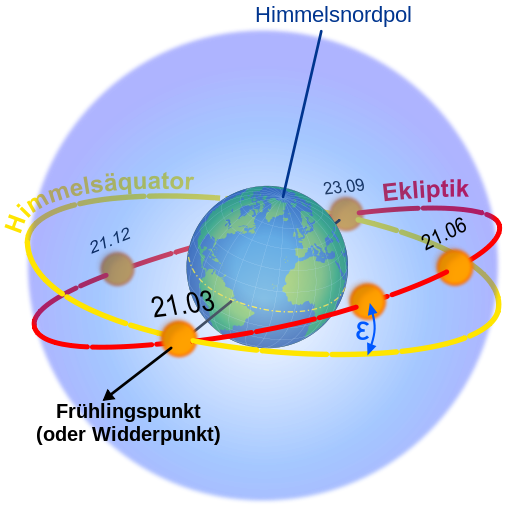
\includegraphics[scale=0.3]{./Bilder/Ecliptic.png}
\caption{\label{fig_Ekliptik}%
\"Aquatorebene und Ekliptik sind um $23,44^\circ$ gegeneinander geneigt (hier mit
$\varepsilon$ bezeichnet). Eine
gleichm\"a\ss ige Bewegung der Sonne entlang der Ekliptik wird zu einer
ungleichm\"a\ss igen Bewegung in Bezug auf die L\"angengrade.} 
\end{SCfigure}

In Bezug auf ein solches Koordinatensystem bewegt sich die Sonne im Verlauf eines Jahres
gleichf\"ormig auf einem Kreis, der um $23,44^\circ$ relativ zur \"Aquatorebene geneigt ist. 
Die Gleichf\"ormigkeit dieser Bewegung folgt aus der gleichf\"ormigen Bewegung der Erde um
die Sonne (da wir eine Kreisbewegung annehmen). Die L\"angengrade auf der Erde schneiden
die scheinbare Bahn der Sonne, die relativ zum \"Aquator geneigt ist, jedoch nicht gleichf\"ormig.
Das bedeutet, dass die scheinbare Bewegung der Sonne relativ zu den L\"angengraden
nicht gleichf\"ormig ist, und das wiederum bedeutet, dass ein Sonnentag zu manchen Zeiten
k\"urzer bzw.\ l\"anger ist. Genauer sind die Tage um den Fr\"uhlings- und Herbstpunkt die
k\"urzesten und die Tage um die Sommer- und Wintersonnenwende die l\"angsten.  
 
Zur Berechnung dieses Effekts f\"ur die Zeitgleichung 
muss man einen gleichm\"a\ss ig unterteilten Vollkreis, der unter $23,44^\circ$ geneigt ist,
entlang der L\"angengrade auf die \"Aquatorebene projizieren. 
Die auf der Ekliptik gleichen\index{Sommersonnenwende}\index{Wintersonnenwende}
Bogenl\"angen werden auf der \"Aquatorebene ungleich - etwas dichter am Fr\"uhlingspunkt (derzeit
21.3.) und Herbstpunkt (derzeit 23.9.) und etwas weniger dicht bei der Sommersonnenwende
(derzeit 21.6.) und der Wintersonnenwende 
(derzeit 21.12).\index{Fruehlingspunkt@Fr\"uhlingspunkt}\index{Herbstpunkt}      
   
\begin{figure}[htb]
\begin{picture}(200,100)(0,0)
\put(135,54){\makebox(0,0){${\scriptstyle 23,44^\circ}$}}
\put(175,75){\makebox(0,0){$\bullet$}}
\put(175,50){\makebox(0,0){$\bullet$}}
\put(100,50){\makebox(0,0){$\bullet$}}
\put(145,73){\makebox(0,0){$a$}}
\put(147,43){\makebox(0,0){$a'$}}
\put(50,20){\makebox(0,0){\footnotesize Ekliptik}}
\put(30,57){\makebox(0,0){\footnotesize \"Aquator}}
\put(160,15){\makebox(0,0){\footnotesize L\"angengrad}}
\put(175,20){\line(0,1){70}}
\put(100,20){\line(0,1){70}}
\qbezier(148,66)(150,60)(150,50)
\thicklines
\put(10,50){\line(1,0){180}}
\put(10,20){\line(3,1){180}}
\end{picture}
\hfill
%
\begin{picture}(210,100)(0,0)
\put(190,20){\makebox(0,0){${\scriptstyle 0^\circ}$}}
\put(185,85){\makebox(0,0){${\scriptstyle 23,44^\circ}$}}
\put(45,20){\makebox(0,0){$\bullet$}}
\put(155,20){\makebox(0,0){$\bullet$}}
\put(50,81){\makebox(0,0){$\bullet$}}
\put(150,81){\makebox(0,0){$\bullet$}}
\put(100,77){\makebox(0,0){$a$}}
\put(100,27){\makebox(0,0){$a'$}}
\put(10,83){\line(1,0){160}}
\qbezier(52,95)(45,60)(45,20)
\qbezier(148,95)(155,60)(155,20)
\put(25,72){\makebox(0,0){\footnotesize Ekliptik}}
\put(30,13){\makebox(0,0){\footnotesize \"Aquator}}
\put(180,50){\makebox(0,0){\footnotesize L\"angengrad}}
\thicklines
\put(10,20){\line(1,0){170}}
\qbezier(10,80)(100,85)(190,80)
\end{picture}
\caption{\label{fig_ZGProj}%
Projektionen von der Ekliptik auf die \"Aquatorebene in der N\"ahe der \"Aquinoktien (Schnittpunkte
zwischen \"Aquator und Ekliptik; links) und der Sommer- bzw.\ Wintersonnenwende (rechts). Zwei Punkte,
die entlang der Ekliptik eine Bogenl\"ange $a$ haben, werden entlang der L\"angengrade auf zwei
Punkte auf dem \"Aquator projiziert, die dort eine Bogenl\"ange $a'$ haben. Man vergleiche diese
Abbildung auch mit Abb.\ \ref{fig_Hondius1} und \ref{fig_Hondius2}.}
\end{figure}   
   
Die folgende Herleitung dieses Beitrags geht davon aus, dass sich der Effekt wieder als
eine trigonmetrische Funktion schreiben l\"asst, was in guter N\"aherung auch erf\"ullt ist. 
Diese Funktion hat im Verlaufe eines Jahres zwei Maxima (an den Sonnenwenden) und zwei
Minima (an den \"Aquinoktien). Damit m\"ussen wir nur noch die Amplitude dieser Funktion
bestimmen.   

Wie aus Abb.\ \ref{fig_ZGProj} ersichtlich, \"andert sich eine Bogenl\"ange $a$, wenn sie von der
Ekliptik entlang der L\"angengrade auf den \"Aquator projiziert wird. In der N\"ahe der
\"Aquinoktien ist die Beziehung durch $a'= a \cos \varepsilon$ gegeben. In der N\"ahe der
Sonnenwendepunkte am $23,44$.ten Breitengrad gilt ungef\"ahr 
\mbox{$a=a' \cos \varepsilon$} (genauer
ist dies die Beziehung zwischen den Bogenl\"angen entlang der beiden Breitengrade; der
Abstand zwischen den beiden Punkten entlang der Ekliptik ist etwas kleiner, dies kann man aber
in f\"uhrender Ordnung und wenn die Punkte gen\"ugend nahe beieinander liegen vernachl\"assigen).   
Machen wir wieder einen Ansatz der Form
\begin{equation}
                \alpha(t) = \alpha_0 \left( 1 + B \cos \left( \frac{4 \pi}{T} t \right) \right) 
\end{equation}
folgt   
\begin{equation}
                \frac{\alpha_{\rm min}}{\alpha_{\rm max}}  
                =  \frac{ 1 - B}{1+B} = \cos^2 \varepsilon  
\end{equation}
oder
\begin{equation}
               B =  \frac{ 1 - \cos^2 \varepsilon }{1+\cos^2 \varepsilon } =  0,0859153\, . 
\end{equation}
Dies f\"uhrt auf maximale Schwankungen in der Tagesl\"ange von $\pm 20,27$\,s und auf
eine kumulative Zeitverschiebung von 
\begin{equation}
     {\rm ZG}_2(t) = \sum_{t=0}^t \Delta T(t)  \approx  \frac{T}{4\pi} \Delta T \sin \frac{4\pi}{T}t  
                    \approx (9,82\,{\rm min})\cdot \sin \frac{4\pi}{T}t  \, .
\end{equation}
Wiederum ist $T$ die Zeitdauer von einem Jahr, und da in der Summe die Diskretisierung
in Tagen $t$ vorgenommen wurde, sollte auch $T$ in Tagen angegeben werden. 
$t$ ist die Anzahl der Tage vom Fr\"uhlingspunkt (dort ist nun $t=0$) gemessen.

\section{Die Zeitgleichung}

Die Zeitgleichung ist die Summe dieser beiden Beitr\"age. Dabei ist noch zu ber\"ucksichtigen,
dass die Zeitpunkte $t=0$ unterschiedlich gew\"ahlt wurden. Gibt man $t$ in Tagen an, sollte
die Periode f\"ur den ersten Anteil (elliptische Erdbahn) am 3.\ Januar beginnen, also am 3.\ Tag
des Jahres, und die Periode f\"ur den zweiten Anteil (Neigung der Erdachse zur Ekliptik) am
21.\ M\"arz, in Jahren, die kein Schaltjahr sind, also am 80.\ Tag eines Jahres. 
Abb.\ \ref{fig_Zeitgleichung} zeigt die Summe der beiden Beitr\"age.

\begin{SCfigure}[30][htb]
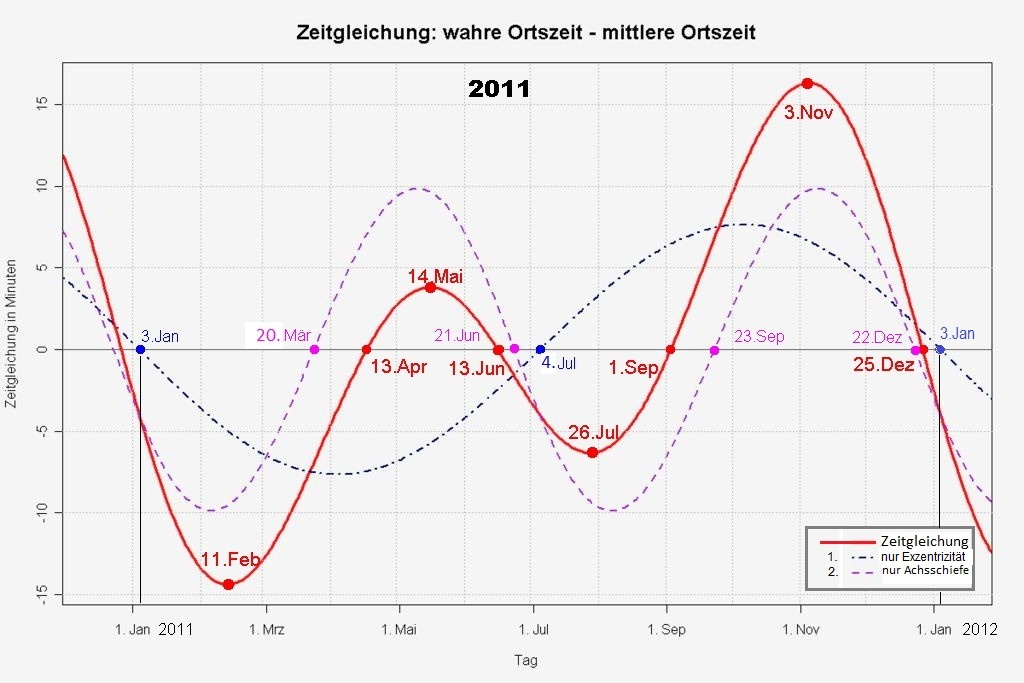
\includegraphics[scale=0.36]{./Bilder/Zeitgleichung.jpg}
\caption{\label{fig_Zeitgleichung}%
Die Zeitgleichung. Im Verlaufe eines Jahres kann die wahre Ortszeit von der mittleren Ortszeit
um \"uber eine Viertelstunde abweichen. Da sich das Perihel langsam verschiebt (in rund 21\,000 Jahren
einmal um $360^\circ$) verschieben sich im Verlauf der Zeit auch die beiden Beitr\"age relativ zueinander.
(aus \cite{Wikipedia_Zeitgleichung})} 
\end{SCfigure}

Insgesamt sind die Minuten der Zeitgleichung zur wahren Ortszeit zu addieren, sodass man die
mittlere Ortszeit erh\"alt. Diese Wahl des Vorzeichens geht darauf zur\"uck, dass man fr\"uher
beispielsweise mithilfe eines Sextanten auf hoher See die wahre Ortszeit gemessen hat
und nun die mittlere Ortszeit berechnen musste. 
Ist die Zeitgleichung negativ (beispielsweise zu Beginn des Jahres) m\"ussen die 
entsprechenden Minuten (Absolutwerte) der Zeitgleichung also von der wahren Ortszeit 
abgezogen werden, um zur mittleren Ortszeit zu gelangen. 

\section{Kuriosit\"aten}
\subsection{Die Ekliptik auf alten Landkarten und Globen}

Auf manchen alten Landkarten und Globen ist die Projektion der Ekliptik auf die
Erde eingezeichnet. Ein Beispiel ist die bekannte Weltkarte von\index{Hondius, Hendrik} 
Hendrik Hondius aus dem
Jahr 1630 (Abb.\ \ref{fig_Hondius}, oben).

\begin{figure}[p]
\includegraphics[scale=0.44]{./Bilder/Hondius_gesamt.png}\\[0.2cm]
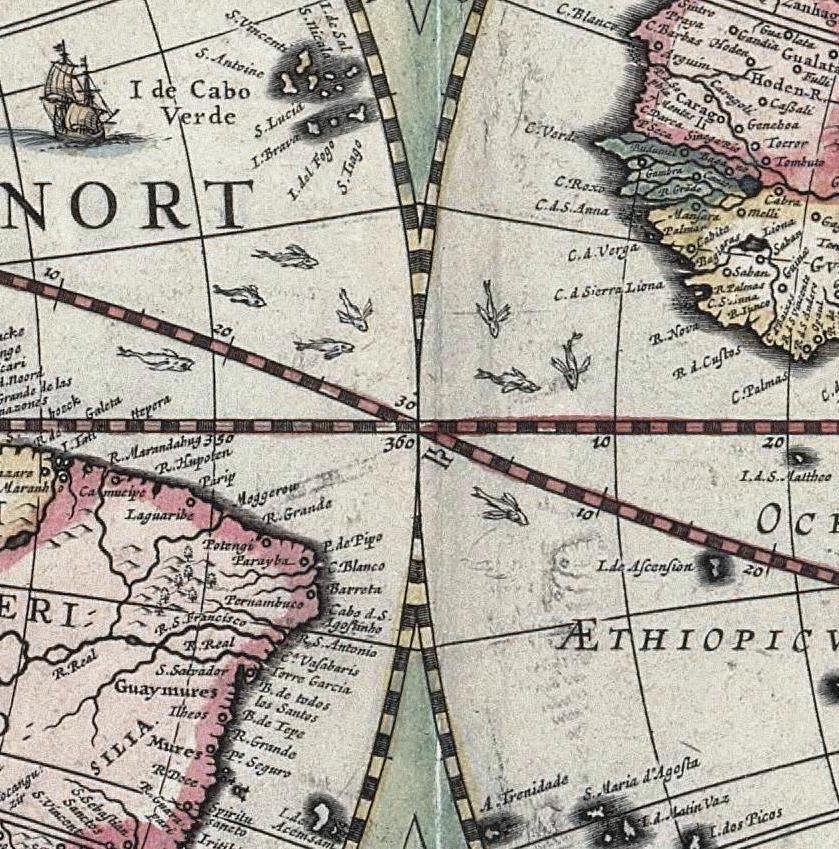
\includegraphics[scale=0.2]{./Bilder/Hondius_00.jpg} \hfill
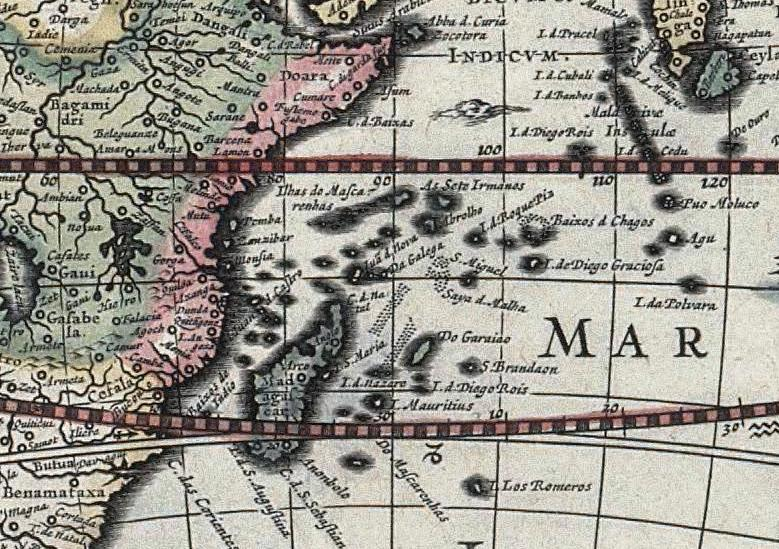
\includegraphics[scale=0.31]{./Bilder/Hondius_90.jpg}
\caption{\label{fig_Hondius}%
(Oben) Weltkarte von Hendrik Hondius aus dem Jahr 1630. Deutlich erkennbar neben der
\"Aquatorlinie ist die Projektion der Ekliptik. (Unten)
Ausschnitte aus der Weltkarte von Hendrik Hondius. (links) Ausschnitt beim Schnittpunkt von 
\"Aquator und Ekliptik, der hier auf einen der damals gebr\"auchlichen Nullmeridiane durch die
Azoren gelegt wurde. Links unten sind Teile von S\"udamerika erkennbar, rechts oben Teile von
Afrika. (rechts) Ausschnitt in der N\"ahe des s\"udlichen Wendepunkts der Ekliptik (unser
Winterpunkt). Der Kontinent links ist Afrika, die Insel rechts daneben Madagaskar; rechts oben
erkennt man die S\"udspitze von Indien und Sri Lanka (damals Ceylon). (\cite{Puzzle})}
\end{figure}

Sowohl die \"Aquatorlinie als auch die Ekliptik sind in $360$ \"aquidistante Einheiten von
jeweils $1^\circ$ unterteilt. F\"ur die \"Aquatorlinie gilt das auch auf der Karte. Da der Gro\ss kreis
der Ekliptik in seiner Projektion auf der Karte bei unterschiedlichen Breitengraden verl\"auft und
der Ma\ss stab der Karte vom Breitengrad abh\"angt (siehe auch Kap.\ \ref{chap_Landkarte}),
erscheint die Unterteilung der Ekliptik nicht mehr gleichf\"ormig.
In der N\"ahe der Wendepunkten der Sonne, also in den Bereichen, wo die
Ekliptik in der N\"ahe des $\pm 23,5$.\ Breitengrads ist, sind die Unterteilungen auf der Ekliptik etwas
breiter als am \"Aquator (siehe Abb.\ \ref{fig_Hondius}, unten rechts), da der Ma\ss stab auf der Karte kleiner
wird, wenn man sich vom \"Aquator entfernt. In den Ausschnitten (Abb.\ \ref{fig_Hondius}, unten)
erkennt man, dass beim Schnittpunkt der Ekliptik mit dem \"Aquator (also den \"Aquinoktien) die
Projektion der Ekliptik auf den \"Aquator die Bogenl\"ange schrumpfen l\"asst (Abb.\ \ref{fig_Hondius}, unten links).
An diesen Stellen schneidet die $10^\circ$ Bogenl\"ange der Ekliptik den \"Aquator links von der
$10^\circ$ Marke bzw.\ dem 10.\ L\"angengrad. Andererseits vergr\"o\ss ert
wegen des ver\"anderten Ma\ss stabs die Projektion entlang der L\"angengrade in der
N\"ahe der Wendepunkte die Bogenl\"ange (Abb.\ \ref{fig_Hondius}, unten rechts): Hier liegt die
$10^\circ$ Marke der Ekliptik ($10^\circ$ neben dem Wendepunkt) rechts neben dem 100.\ L\"angengrad
(der 90.\ L\"angengrad markiert den Wendepunkt) am \"Aquator. 

\subsection{Das Analemma}
\label{sec_Analemma}

Das Analemma\index{Analemma} 
ist eine achtf\"ormige Figur, die ungef\"ahr den Schattenverlauf der Spitze
eines Stabes (z.B.\ eines Obelisken oder der Spitze des Zeigers einer Sonnenuhr) zur
selben mittleren Ortszeit (z.B.\ um 12 Uhr mittags) im Verlauf eines Jahres beschreibt (siehe
Abb.\ \ref{fig_Analemma}, links). 
Die beiden Koordinaten dieser Figur entsprechen einmal dem unterschiedlichen H\"ochstand
der Sonne im Sommer und Winter: Im Winter steht die Sonne auch zur Mittagszeit sehr tief
und somit ist der Schatten vergleichsweise lang, im Sommer steht die Sonne hoch am
Himmel und daher ist der Schatten entsprechend kurz. 

\begin{figure}[htb]
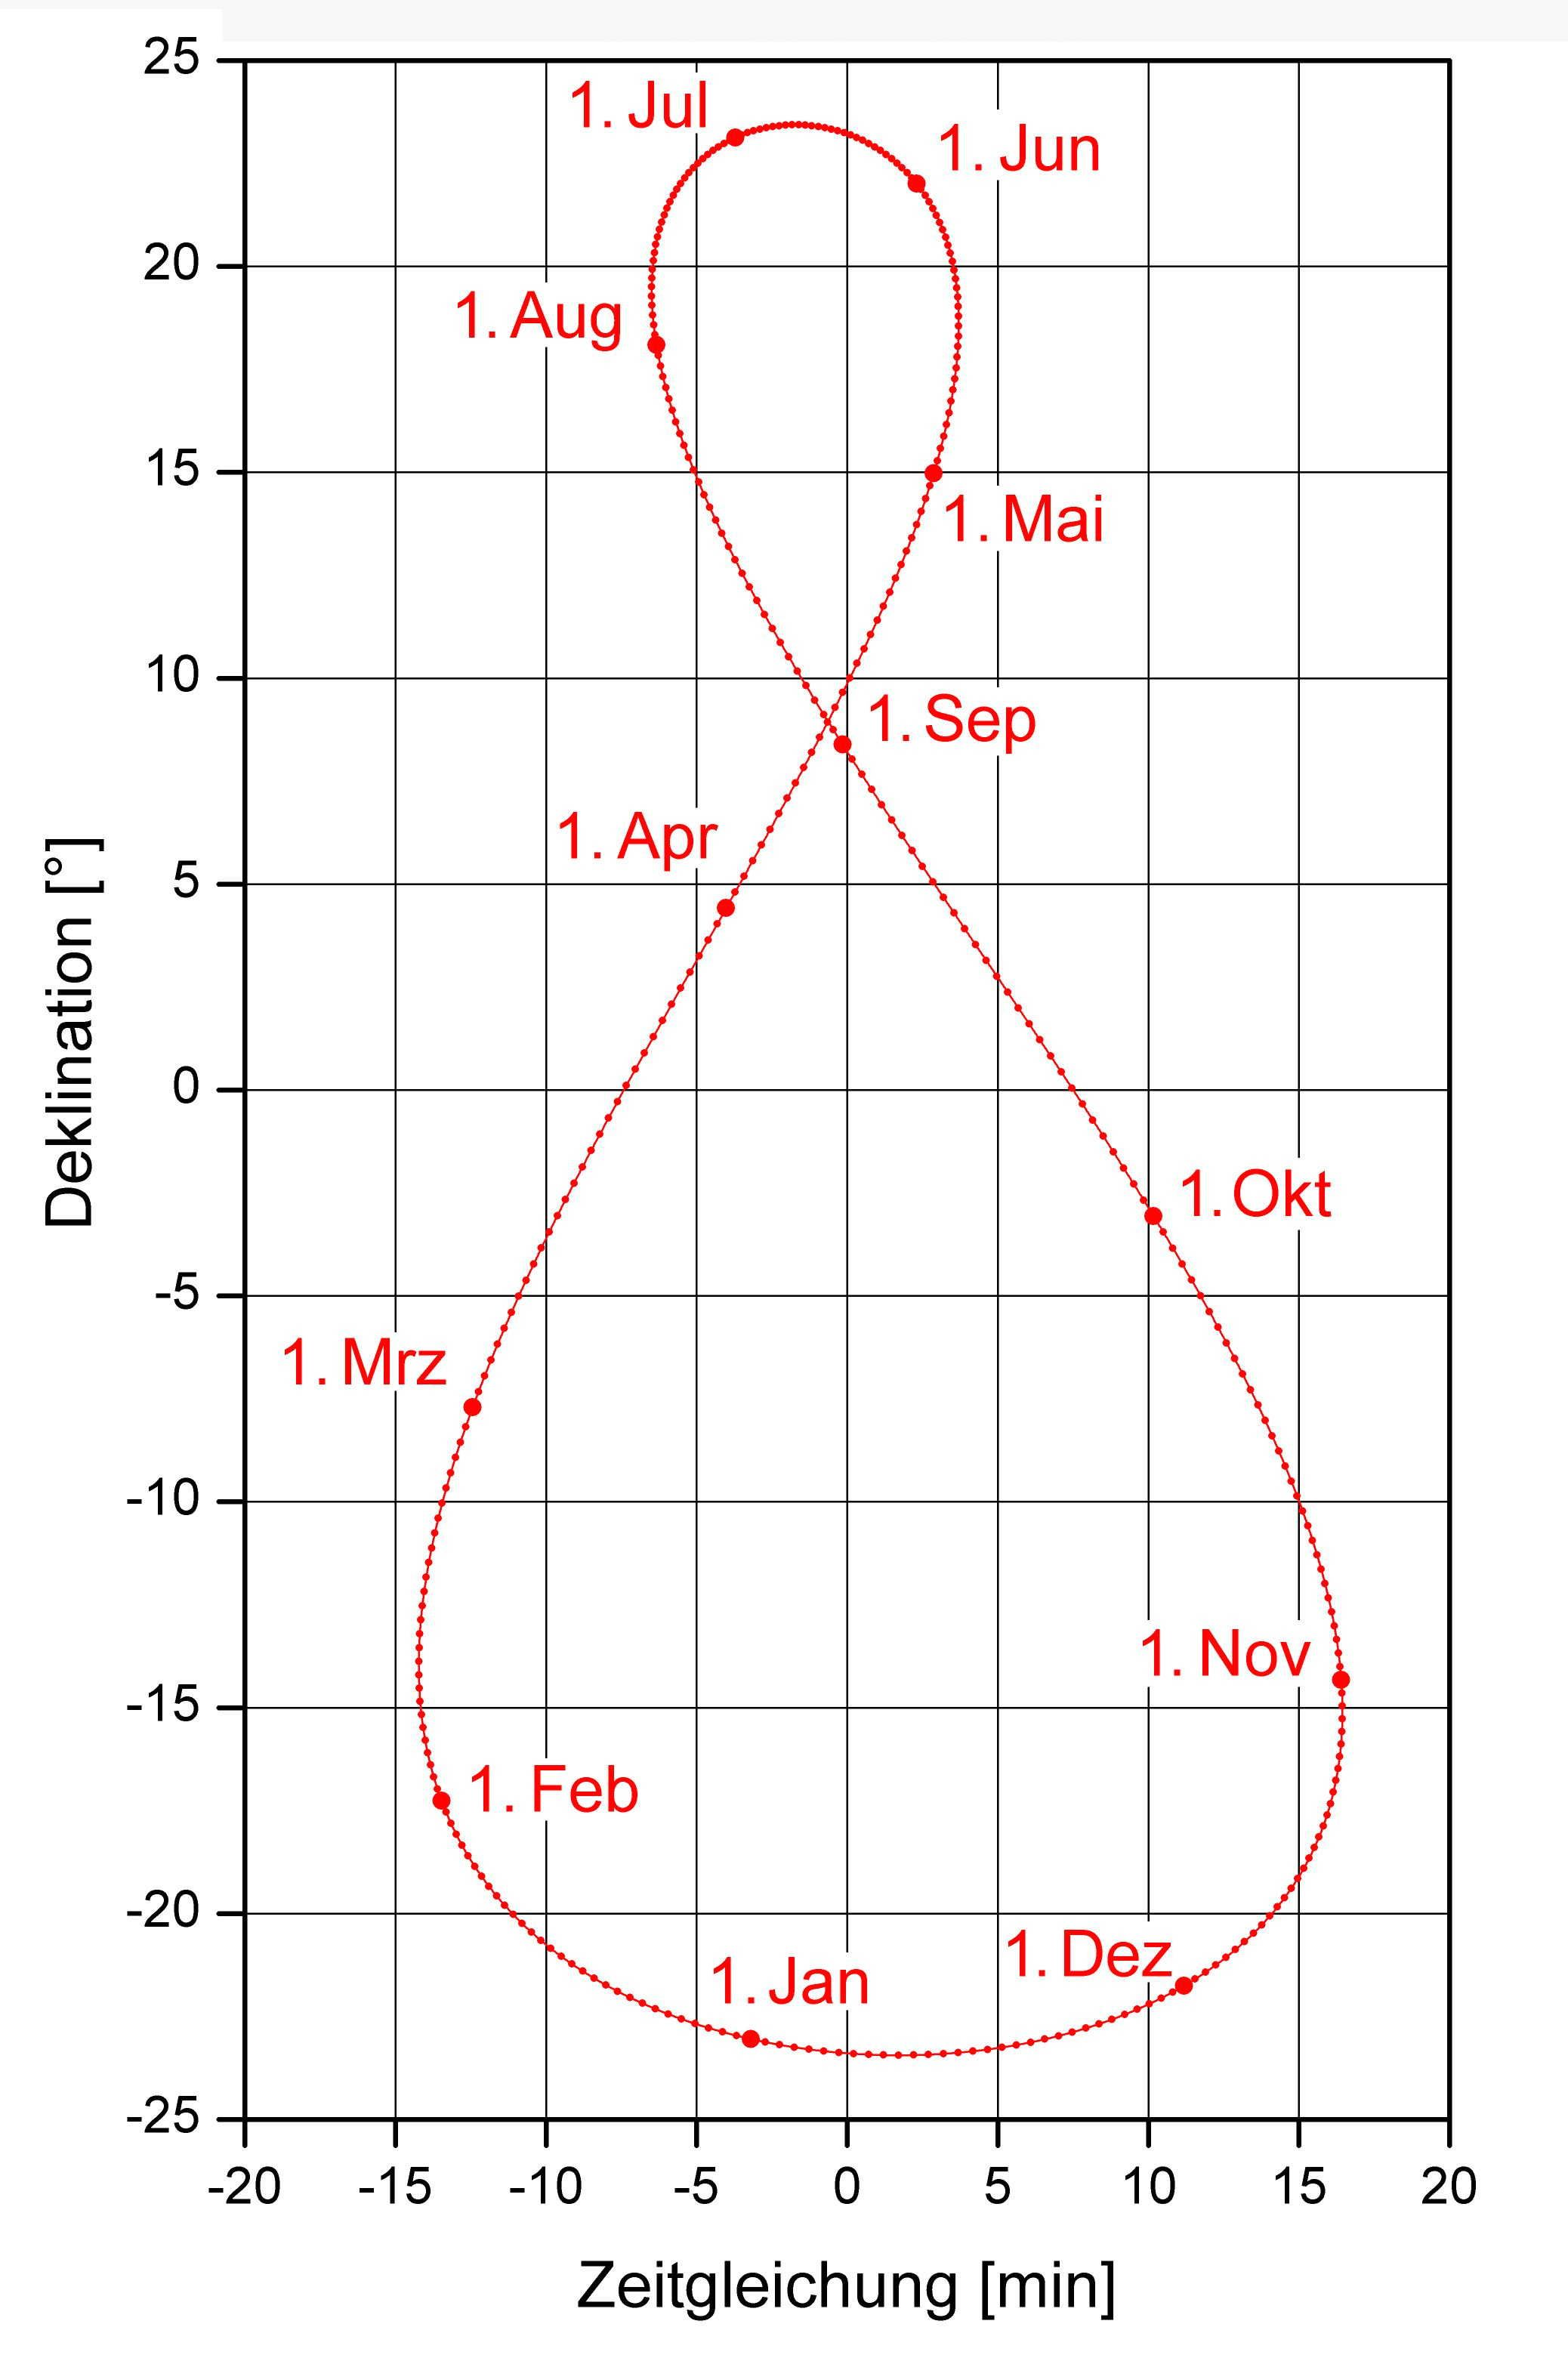
\includegraphics[scale=0.28]{./Bilder/Analemma.jpg} 
\hfill
\includegraphics[scale=0.24]{./Bilder/Munich_Altes_Rathaus_Sundial.jpg}
\caption{\label{fig_Analemma}%
Das Analemma. (links) Die derzeitige Figur des Analemmas. Die obere Spitze der 8
beschreibt den Sonnenstand im Sommer, wenn die Sonne hoch steht und der Schatten
entsprechend kurz ist. Der Zeiger oder Obelisk steht oberhalb der Figur und die S\"udrichtung
ist nach oben (aus \cite{Wikipedia_Analemma}). (rechts) Die Sonnenuhr am Alten Rathaus in M\"unchen
mit einem Analemma zur 
Korrektur der wahren Sonnenzeit auf die mittlere Sonnenzeit. (aus \cite{Niermann})} 
\end{figure}

Die dazu (fast) orthogonale Richtung entspricht der Zeitgleichung: Da die Position der Schattenspitze
immer zur selben mittleren Ortszeit bestimmt wird, geht die wahre Sonne dieser Zeit entsprechend
der Zeitgleichung entweder etwas vor oder nach, d.h.\ der Schatten ist etwas nach links oder
rechts versetzt. 

Manche Sonnenuhren korrigieren den Effekt der Zeitgleichung. Dazu gibt es unterschiedliche
Verfahren. Man kann z.B.\ die Schattenlinien zu einer festen Uhrzeit nicht als Geraden zeichnen
(die einem festen L\"angengrad entsprechen w\"urden) sondern in Form einer langgestreckten
Acht. Hierbei wird, wie bei all diesen Verfahren, ausgenutzt, dass der Schatten im Winter l\"anger
ist als im Sommer. 

Ein weiteres Verfahren besteht darin, den Schattenstab der Sonnenuhr unterschiedlich dick
zu machen und zum Ablesen an einer Skala eine bestimmte Kante des Schattens zu 
verwenden (siehe Abb.\ \ref{fig_Bernhardt}).
Solche St\"abe bezeichnet man auch als Bernhardt'sche Walze (benannt nach dem Techniker
Martin Bernhardt,\index{Bernhardt'sche Walze} 
der diese Walze patentieren lie\ss, \"ahnliche Ideen hatte aber auch schon
der Engl\"ander John Ryder Oliver Ende des 19.\ Jahrhunderts). 
Ebenfalls wegen der unterschiedlichen Sonnenh\"ohe zu den verschiedenen Jahreszeiten
w\"urde ein jeweils anderer Teil des Schattenstabs den Schatten auf die Skala werfen. Wegen
der unterschiedlichen Dicke erreicht man so, dass diese Schattenkante entsprechend 
verschoben ist. Da die Zeitgleichung in den beiden Jahresh\"alften unterschiedlich ist, ben\"otigt
man einen Schattenstab f\"ur die erste und einen anderen Schattenstab f\"ur die zweite
Jahresh\"alfte.   

\begin{SCfigure}[30][h]
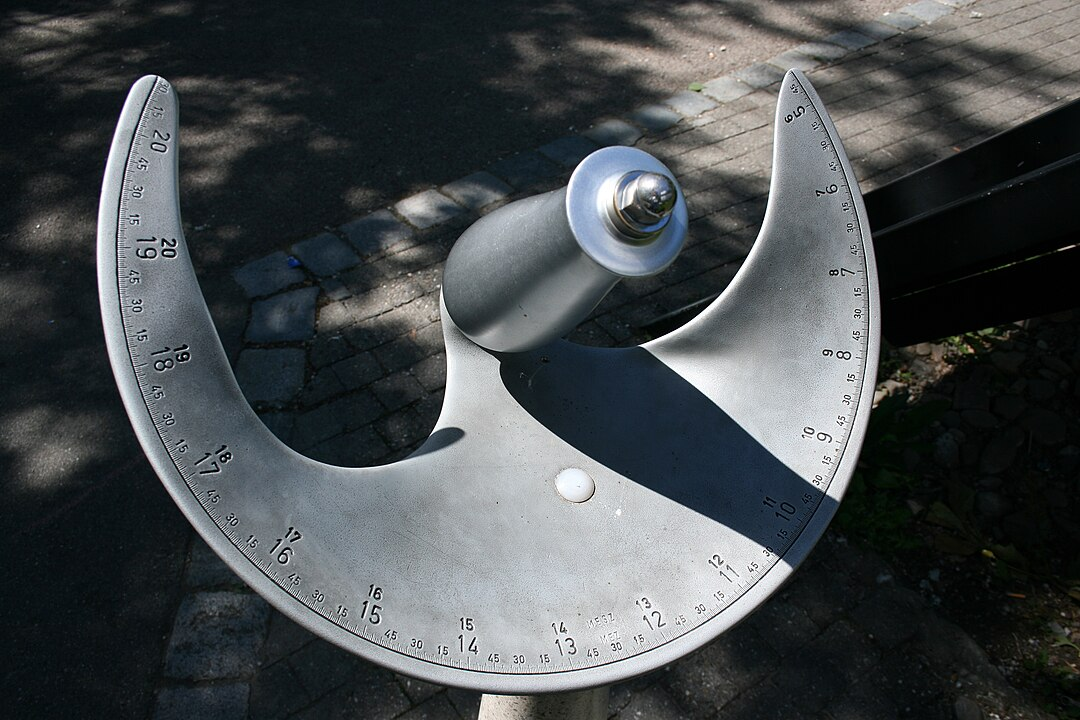
\includegraphics[scale=0.2]{./Bilder/Bernhardt.jpg}
\caption{\label{fig_Bernhardt}%
Sonnenuhr mit Bernhardt'scher Winterwalze. (aus \cite{Wikipedia_Sonnenuhr})}
\end{SCfigure}

Im Verlauf der Zeit verschieben sich die beiden Beitr\"age zur Zeitgleichung gegeneinander. 
W\"ahrend sich der Neigungswinkel zur Ekliptik nur sehr wenig und \"uber einen sehr gro\ss en
Zeitraum von \"uber 40\,000 Jahren ver\"andert, wandert das Perihel im Verlauf von rund 
21\,000 Jahren einmal durch das Jahr. Dadurch ver\"andert sich die Zeitgleichung langsam
und somit auch die Form des Analemmas. Derzeit ist das Analemma leicht asymmetrisch,
weil die Wintersonnenwende und das Perihel nicht auf denselben Tag fallen (das war z.B.\ im
Jahr 1246 der Fall). Au\ss erdem sind die beiden \glqq Hanteln\grqq\ der Acht unterschiedlich 
gro\ss. Wenn das Perihel im Fr\"uhlings- bzw.\ Herbstpunkt steht, sind die beiden Teile
gleich gro\ss.  

\subsection{Der k\"urzeste Tag}

Die Wintersonnenwende entspricht gemeinhin dem k\"urzesten Tag. Derzeit liegt dieses Ereignis
um den 21.\ Dezember.\index{Wintersonnenwende} 
Zu diesem Zeitpunkt befindet sich sie Sonne \"uber dem s\"udlichen
Wendekreis (dem Wendekreis des Steinbocks).\index{Wendekreis des Steinbocks} 
In Freiburg liegen zwischen Sonnenaufgang\index{Freiburg!Sonnenauf-,-untergang}
und Sonnenuntergang an diesem Tag 8 Stunden, 22 Minuten und 13 Sekunden. Doch k\"urzester 
Tag hei\ss t nicht, dass es an diesem Tag am fr\"uhesten dunkel wird oder am sp\"atesten
hell. Der fr\"uheste Sonnenuntergang liegt um den 11.\ Dezember (in Freiburg um 16:35),
der sp\"ateste Sonnenaufgang ist um den 2.\ Januar (in Freiburg gegen 8:18). Alle angegebenen
Uhrzeiten beziehen sich nat\"urlich auf die mittlere Sonnenzeit (genauer MEZ) und nicht die
wahre Sonnenzeit. Der Grund f\"ur den Unterschied ist die Zeitgleichung. 

Eine \"ahnliche Aussage gilt f\"ur die Sommersonnenwende.\index{Sommersonnenwende} 
Der l\"angste Tag mit
16 Stunden 2 Minuten und 47 Sekunden in Freiburg ist der 21.\ Juni. Doch der fr\"uhste Sonnenaufgang
liegt um den 16./17.\ Juni (gegen 5:18), der sp\"ateste Sonnenuntergang um den 25./25.\ Juni (gegen
21:32). Genaue Zeiten f\"ur die Tagesl\"ange, Sonnenauf- und Untergang sowie weitere
interessante Daten f\"ur jeden beliebigen Ort der Erde findet man auf der Webseite \cite{timeanddate}.

\section{Anhang}
\subsection{\"Aquivalenz des zweiten Kepler'schen Gesetzes und der Drehimpulserhaltung}
\label{sec_Zeitgleichung_A}

Sei $\pmb{r}$ der Verbindungsvektor von einem Brennpunkt der Ellipse - dem Brennpunkt, in 
dem sich die Sonne befindet - zu einem Punkt auf der Ellipse (dem Ort eines Planeten)
und $\Delta \pmb{r}$ die in der Zeit $\Delta t$ zur\"uckgelegte Strecke in tangentialer
Richtung. Das zweite Kepler'sche Gesetz\index{Kepler'sches Gesetz!zweites} 
besagt, dass die in dem Zeitraum $\Delta t$ (f\"ur $\Delta t\rightarrow 0$)
\"uberstrichene Fl\"ache $\Delta F$, d.h.
\begin{equation}
                    \Delta F = \frac{1}{2} \pmb{r} \times \Delta \pmb{r} \, ,
\end{equation} 
entlang der Bahnkurve immer gleich ist. Damit ist aber auch der Drehimpuls
\begin{equation}
                    \pmb{L} = m  \pmb{r} \times \frac{{\rm d} \pmb{r}}{{\rm d} t} 
\end{equation} 
konstant.\index{Drehimpulserhaltung}
Das Argument gilt nat\"urlich auch in der umgekehrten Richtung: Aus der
Drehimpulserhaltung folgt das zweite Kepler'sche Gesetz.


\begin{thebibliography}{99}
\bibitem{Wikipedia_Analemma} aus Wikipedia \glqq Analemma\grqq; S.\ Wetzel, CC BY-SA 4.0.
\bibitem{Niermann} Till Niermann - Eigenes Werk, CC BY-SA 3.0, 
                \url{https://commons.wikimedia.org/w/index.php?curid=21792620}
\bibitem{Puzzle} Ravensburger Puzzle; Antique World Map, Hondius.                 
\bibitem{timeanddate} 
   {\small \verb+https://www.timeanddate.com/sun/germany/freiburg+} 
\bibitem{Wikipedia_Sonnenuhr} Wikipedia \glqq Sonnenuhr\grqq; 
           Pr\"azisions-Sonnenuhr mit Winterwalze am Carl Zeiss Planetarium, Stuttgart.
           \url{https://de.wikipedia.org/wiki/Sonnenuhr}   
\bibitem{Wikipedia_Zeitgleichung} Wikipedia \glqq Zeitgleichung\grqq; 
                 \url{https://de.wikipedia.org/wiki/Zeitgleichung} (aufgerufen am 14.5.2023).
\bibitem{Wikipedia_Zeitzone} Wikipedia \glqq Zeitzone\grqq. \url{https://de.wikipedia.org/wiki/Zeitzone}
\end{thebibliography}


%\end{document}

